\hypertarget{tcp-ip-ux7b80ux4ecb}{%
\subsection{TCP IP 简介}\label{tcp-ip-ux7b80ux4ecb}}

虽然大家现在对互联网很熟悉,但是计算机网络的出现比互联网要早很多。

计算机为了联网,就必须规定通信协议,早期的计算机网络,都是由各厂商自己规定一套协议,IBM、Apple
和 Microsoft
都有各自的网络协议,互不兼容,这就好比一群人有的说英语,有的说中文,有的说德语,说同一种语言的人可以交流,不同的语言之间就不行了。

为了把全世界的所有不同类型的计算机都连接起来,就必须规定一套全球通用的协议,为了实现互联网这个目标,互联网协议簇(Internet
Protocol Suite)就是通用协议标准。Internet 是由 inter 和 net
两个单词组合起来的,原意就是连接 ``网络'' 的网络,有了
Internet,任何私有网络,只要支持这个协议,就可以联入互联网。

因为互联网协议包含了上百种协议标准,但是最重要的两个协议是 TCP 和 IP
协议,所以,大家把互联网的协议简称 TCP/IP 协议。

通信的时候,双方必须知道对方的标识,好比发邮件必须知道对方的邮件地址。互联网上每个计算机的唯一标识就是
IP
地址,类似\texttt{123.123.123.123}。如果一台计算机同时接入到两个或更多的网络,比如路由器,它就会有两个或多个
IP 地址,所以,IP 地址对应的实际上是计算机的网络接口,通常是网卡。

IP
协议负责把数据从一台计算机通过网络发送到另一台计算机。数据被分割成一小块一小块,然后通过
IP
包发送出去。由于互联网链路复杂,两台计算机之间经常有多条线路,因此,路由器就负责决定如何把一个
IP 包转发出去。IP
包的特点是按块发送,途径多个路由,但不保证能到达,也不保证顺序到达。

 
 \begin{figure}[htp]
	\centering
	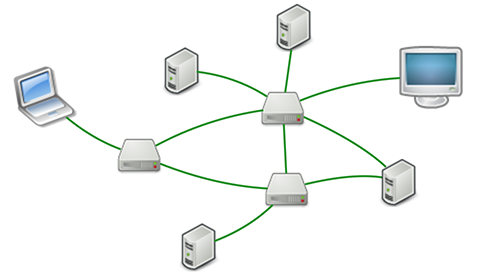
\includegraphics[width=0.6\linewidth]{fig/972515044819040.png}
\end{figure}


IP 地址实际上是一个 32 位整数(称为 IPv4),以字符串表示的 IP
地址如\texttt{192.168.0.1}实际上是把 32 位整数按 8
位分组后的数字表示,目的是便于阅读。

IPv6 地址实际上是一个 128 位整数,它是目前使用的 IPv4
的升级版,以字符串表示类似于\texttt{2001:0db8:85a3:0042:1000:8a2e:0370:7334}。

TCP 协议则是建立在 IP 协议之上的。TCP
协议负责在两台计算机之间建立可靠连接,保证数据包按顺序到达。TCP
协议会通过握手建立连接,然后,对每个 IP
包编号,确保对方按顺序收到,如果包丢掉了,就自动重发。

许多常用的更高级的协议都是建立在 TCP 协议基础上的,比如用于浏览器的 HTTP
协议、发送邮件的 SMTP 协议等。

一个 TCP 报文除了包含要传输的数据外,还包含源 IP 地址和目标 IP
地址,源端口和目标端口。

端口有什么作用?在两台计算机通信时,只发 IP
地址是不够的,因为同一台计算机上跑着多个网络程序。一个 TCP
报文来了之后,到底是交给浏览器还是
QQ,就需要端口号来区分。每个网络程序都向操作系统申请唯一的端口号,这样,两个进程在两台计算机之间建立网络连接就需要各自的
IP 地址和各自的端口号。

一个进程也可能同时与多个计算机建立链接,因此它会申请很多端口。

了解了 TCP/IP 协议的基本概念,IP
地址和端口的概念,我们就可以开始进行网络编程了。

